\mychapter{Case Study: Design of Vehicle Suspensions\label{ch:8}}

%--- epigraph
\epigraph{\textit{``Systems engineering should be, first and foremost, a state of mind and an attitude taken when dealing with complexity.''}}{\textmd{J.-L. Wippler} \cite[p.~208]{Luzeaux2013a}}
%--- epigraph

%-----------------------------------------
\section{Introduction\label{sec:ch8:introduction}}

The design of vehicle suspensions has been of considerable interest ever since the invention of the automobile.
A suspension transfers forces in the system to provide a smooth ride for the passenger and good handling characteristics among other objectives.
Fundamentally, it is a type of vibration isolator \cite{Kasturi1998a, Hrovat1997a, Hrovat1993a} .
Different types of suspensions can typically be classified into the three categories of passive \cite{Kasturi1998a, Gobbi2001a, He2005a, Allison2008b, Hrovat1997a, Hrovat1993a}, semi-active \cite{Deshmukh2015a, Koch2014a, Hrovat1993a, Bourmistrova2005a}, or active \cite{Fathy2003a, Alyaqout2007b, Allison2014b, Hrovat1997a, Ulsoy1994a, Hrovat1993a} depending on the external energy flow into the system. 
There has been considerable research interest in analyzing and optimizing all types of suspensions, particularly utilizing tools from dynamics and controls.
However, much of this research has focused on a select few canonical suspensions such as the ones shown in Figs.~\ref{fig:ch8:csuspension1}--\ref{fig:ch8:csuspension4}. 
Here we will consider architecture changes in the suspensions, i.e.,~different components connected in new ways, such as the suspensions shown in Figs.~\ref{fig:ch8:csuspension5}--\ref{fig:ch8:csuspension6}.
In all the suspensions, an unsprung mass \xcolor{U} is connected to the road profile \gls{road}, and there is some mechanical path between the sprung mass \xcolor{S} and \xcolor{U}.

\begin{figure}
\centering

\begin{subfigure}[t]{0.33\textwidth}
\centering
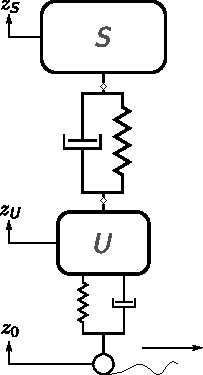
\includegraphics[scale=0.8]{../ch8/figures/csuspension1}
\caption{Canonical passive \cite{Allison2008b, Gobbi2001a}.\label{fig:ch8:csuspension1}}
\end{subfigure}%
\begin{subfigure}[t]{0.33\textwidth}
\centering
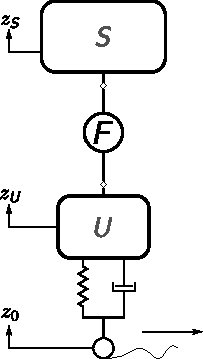
\includegraphics[scale=0.8]{../ch8/figures/csuspension2}
\caption{Pure active \cite{Hrovat1993a, Hrovat1997a}.\label{fig:ch8:csuspension2}}
\end{subfigure}%
\begin{subfigure}[t]{0.33\textwidth}
\centering
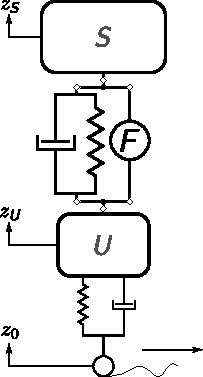
\includegraphics[scale=0.8]{../ch8/figures/csuspension3}
\caption{Canonical active \cite{Allison2014b, Alyaqout2007b, Fathy2003a, He2005a, Ulsoy1994a}.\label{fig:ch8:csuspension3}}
\end{subfigure}%

\vspace{0.1in}

\begin{subfigure}[t]{0.33\textwidth}
\centering
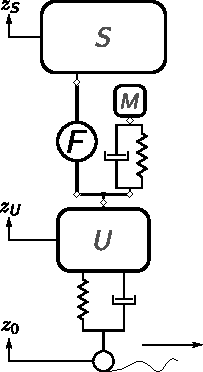
\includegraphics[scale=0.8]{../ch8/figures/csuspension4}
\caption{Active with dynamic absorber \cite{Hrovat1993a, Hrovat1997a}.\label{fig:ch8:csuspension4}}
\end{subfigure}%
\begin{subfigure}[t]{0.33\textwidth}
\centering
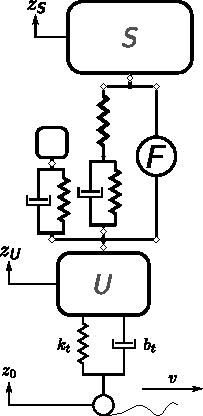
\includegraphics[scale=0.8]{../ch8/figures/csuspension5}
\caption{Active candidate.\label{fig:ch8:csuspension5}}
\end{subfigure}%
\begin{subfigure}[t]{0.33\textwidth}
\centering
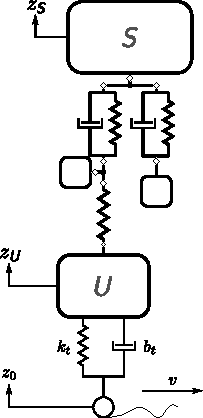
\includegraphics[scale=0.8]{../ch8/figures/csuspension6}
\caption{Passive candidate.\label{fig:ch8:csuspension6}}
\end{subfigure}%

\caption{Various vehicle suspension architectures.\label{fig:ch8:suspensions}}

\end{figure}

% new paragraph
In addition to architecture design changes, both the physical and control system designs will also be considered.
This leads to a complex, challenging design problem that is typically not treated in a systematic fashion in engineering design practice.
Here we will describe a particular problem class of combined architecture, plant, and control problems that can leverage a number of previously developed tools to provide solutions to this design problem.
Due to the breadth of this design study, many simplifying assumptions must be made to keep the problem tractable, but still makes it possible to reveal various design insights.
It has been observed by experts in the field that even simple suspension models and studies have had a ``profound impact on the practical implementations some 15--20 years later \cite{Hrovat1993a}''.
In addition, suspension design problems have proven to be an interesting area for research in combined plant and control design or co-design \cite{Allison2014b, Alyaqout2007b, Fathy2003a}.
It is important to note that the purpose of the early-stage studies proposed in this chapter is not to supplant the detailed, rigorous, robust previous research, but rather seeks to identify new architectures that could be investigated in the same level of detail that the few canonical architectures have received. 

% new paragraph
The remainder of this chapter is organized as follows.
Section~\ref{sec:ch8:class} outlines the considered problem class with linear physical elements.
Section~\ref{sec:ch8:formulation} provides the combined architecture, plant, and control vehicle suspension design problem formulation.
Section~\ref{sec:ch8:results} presents the results of this case study.

%-----------------------------------------

\section{A Problem Class with Linear Physical Elements\label{sec:ch8:class}}

\newcommand{\xarch}{^{(i)}}
\newcommand{\xclass}{^{\mathcal{P}}}

%----------------------------------------------
\subsection{Linear Physical Elements\label{sec:ch8:linearelements}}

A useful framework for describing linear physical elements is bond graph modeling with power port nodes (or simply power nodes) \cite{Borutzky2010a}.
Power nodes are characterized by constitutive parameters and follow some constitutive relation (typically a fundamental physical law).
They can be classified as source nodes (\xcolor{Se}, \xcolor{Sf}), storage nodes (\xcolor{C}, \xcolor{I}),  resistive nodes (\xcolor{R}), reversible transducers (\xcolor{TF}, \xcolor{GY}), and junction nodes (\xcolor{0}, \xcolor{1}).
Some analogies for these power nodes in different energy domains are in Table~\ref{tb:ch8:analogies}.
An example of a \xcolor{TF} (transformer) is a lever, gear, or hydraulic cylinder.
The \xcolor{GY} (gyrator) typically describes the conversion between energy domains, such as with an electrical DC motor or mass accelerometer.
The \xcolor{0}-junction is analogous to Kirchhoff's current law and the \xcolor{1}-junction is analogous to the voltage law in electrical systems.
For more details on bond graph modeling, see Refs.~\cite{Borutzky2010a,Kypuros2013a, Karnopp2012a}

\begin{table}
\centering
\begin{tabular}{cccc}
\hline \hline
& \multicolumn{2}{c}{Linear Mechanical} & \\
Label & Intuitive & Topology Preserving & Electrical \\
\hline
\xcolor{Se} & Force & Velocity & Voltage  \\
\xcolor{Sf} & Velocity & Force & Current \\
\xcolor{C} & $1/K$ & $M$ & $C$  \\
\xcolor{I} & $M$ & $1/K$ & $I$ \\
\xcolor{R} & $B$ & $1/B$ & $R$ \\
\hline \hline
\end{tabular}
\caption{Some bond graph modeling analogies.\label{tb:ch8:analogies}}
\end{table}

The key property for systems represented by bond graphs with \glsfoo[noindex]{LTI} elements is that the equations of motion can be represented as a linear descriptor model.
If we denote the set of all constitutive parameters for a particular bond graph as \gls{parameters}, the model is of the form:
\begin{align}
\gls{dynE}(\bm{p}) \dot{\glsfoo[noindex]{timederiv}\gls{states}} = \gls{dynA}(\bm{p}) \bm{\xi} + \gls{dynB}(\bm{p}) \gls{sources}
\end{align} 

\noindent where $\bm{\xi}$ are the states and $\bm{s}$ are the sources.
The matrix $\bm{E}$ is invertible if there are no algebraic loops in the system \cite{Gonzalez2008a, Borutzky2010a}.
Here we assume that all algebraic loops are appropriately removed (e.g.,~see Ref.~\cite{Gonzalez2008a}) so that we have an explicit first-order \glsfoo[noindex]{ODE} with only $\{\bm{A}, \bm{B}\}$.

% new paragraph
The architecture design decisions will include what power nodes to include in the system and their connections.
The constitutive parameters will be the plant design variables (but the plant design could consist of more realistic variables such as the geometry of spring with a mapping back to the appropriate constitutive parameter).
The control decisions will come in the form of certain source types.
The sources may also be used to add various disturbances to the system.

%----------------------------------------------
\subsection{Problem Class Definition}

We would like to solve architecture design problems of the following form:
\begin{subequations}
\label{eq:ch8:levela}
\begin{align}
\min_{\gls{x}_{\glsfoo[noindex]{architecture}}} \quad & \gls{objective}_a(\bm{x}_a) + \Psi_{\gls{design}}\left( \gls{f}_{\glsfoo[noindex]{plant}}(\bm{x}_a), f_{\glsfoo[noindex]{control}}(\bm{x}_a) \right) \\
\text{subject to:} \quad & f_a(\bm{x}_a) = a \in \gls{feasible}_a
\end{align}
\end{subequations}

\noindent where $\bm{x}_a$ represents architecture design variables, $f_a(\bm{x}_a)$ is a mapping between the architecture design variables and the architecture $a$, and $\mathcal{F}_a$ is the feasible set of architectures.
$\Psi_a$ is the architecture-only objective function (such as a complexity metric that counts the number of additional components \cite{manuscript-pm-circuits}), while $\Psi_d$ is the general design objective function that includes dependence on the plant and control design.
This dependence is represented by the mapping functions $f_p$ and $f_c$ between the architecture and the plant $\bm{x}_p$ and \glsfoo[noindex]{OLC} \gls{olc} design variables. 

% new paragraph
A fair comparison between architecture candidates requires knowledge of the best possible performance for each candidate architecture.
To determine the value of $\Psi_d$ we must solve a suitable co-design problem.
This problem has the following form:
\begin{subequations}
\label{eq:ch8:codesign}
\begin{align}
\min_{\bm{x}_p^{\glsfirst{iarchitecture}}, \bm{u}\xarch} \quad & \Psi_d = \int_{\gls{time}_{\glsfoo[noindex]{initial}}}^{t_{\glsfoo[noindex]{final}}} \gls{lagrange}^{\glsfirst{class}}\left(t, \gls{output}, \bm{x}_p\xarch \right) dt + \gls{mayer}\xclass\left( \bm{y}(t_0), \bm{y}(t_f), \bm{x}_p\xarch \right) \\
\text{subject to:} \quad & \left[ \dot{\bm{\xi}} = \bm{f}\xclass\left( t, \bm{\xi}, \bm{u}, \bm{x}_p \right) \right]\xarch \\
& \gls{equality}\xclass\left(t, \bm{y}, \bm{x}_p\xarch \right) = \bm{0} \\
& \gls{inequality}\xclass\left(t, \bm{y}, \bm{x}_p\xarch \right) \leq \bm{0} \\
\text{where:} \quad & \bm{y} = \bm{y}\xclass\left( t, \bm{\xi}\xarch, \bm{u}\xarch, \bm{x}_p\xarch \right)
\end{align}
\end{subequations}

\noindent where $\Box\xarch$ indicates a problem formulation element appropriate for the $i$th candidate architecture from Prob.~(\ref{eq:ch8:levela}), $t$ is the time continuum between $t_0$ and $t_f$, and $\bm{y}$ are the (architecture-independent) outputs.
The problem elements $\{\mathcal{L}, \mathcal{M}, \bm{f}, \bm{h}, \bm{g} \}$ represent the Lagrange term, Mayer term, dynamics, equality constraints, and inequality constraints.

% new paragraph
The subscript \gls{problemclass} indicates a particular problem class that the problem elements must be in.
Here we will consider a class whose specific structure can lead to efficient solution strategies, but still covers the combined architecture, plant, and control design problems of interest.
Consider a function, $f\xclass$, in the problem class $\mathcal{P}$ with type $f$ (e.g.,~the type might be Lagrange term or inequality constraints).
Then $f\xclass$ must be a function where for fixed values of $\bm{x}_p\xarch$, $f\xclass$ has an equivalent \glsfoo[noindex]{LQDO} problem element described in Chapter~\ref{ch:5}.
With this specification of $\mathcal{P}$, Prob.~(\ref{eq:ch8:codesign}) is a strong candidate for the nested co-design solution strategy for the reasons discussed in Chapter~\ref{ch:3}, namely an efficient inner-loop strategy for LQDO.
This leads to the following trilevel solution approach.

%----------------------------------------------
\subsection{A Trilevel Solution Approach}

\begin{figure}
\centering
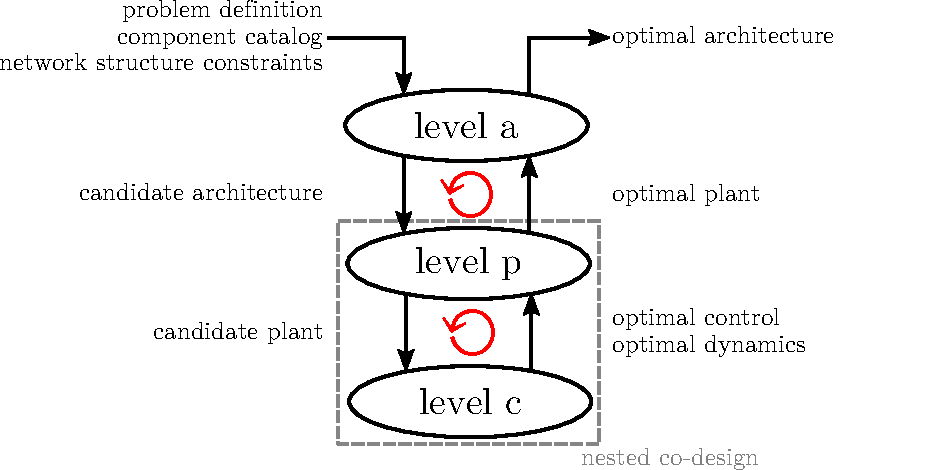
\includegraphics[scale=0.8]{../ch8/figures/trilevel}
\caption{The proposed trilevel solution strategy for combined architecture, plant, and control design.\label{fig:ch8:trilevel}}
\end{figure}

The trilevel solution approach used here is illustrated in Fig.~\ref{fig:ch8:trilevel}.
Each one of the three levels is now described.

\subsubsection{Architecture Design: Level a}

The topmost level is responsible for taking the problem definition, a user-defined component catalog, and network structure constraints and providing candidate architectures for the other levels.
Many architectures can be represented by colored graphs as the nodes in this representation scheme can be used to represent a variety of concepts. 
Therefore, the approach used here will be the perfect matching-based algorithm for generating all architectures in Chapter~\ref{ch:2}.
The different labels in the graphs will correspond to the power nodes in Sec.~\ref{sec:ch8:linearelements}.

\subsubsection{Plant Design: Level p}

The next level takes the candidate architecture and performs the outer-loop co-design tasks for the plant design \cite{Herber2017b}.
The appropriate optimization problem needs to be automatically created and solved.
Since these types of problems can be highly nonconvex (see Chapter~\ref{ch:3}), global search algorithms are utilized to help improve the confidence of finding the true optimal solution (in this chapter, a multistart approach is used, but an alternative is a genetic algorithm \cite{Papalambros2017a, Marti2003a, Eiben2003a}).

% new paragraph
An automated model generation procedure (see Sec.\ref{sec:ch1:modelgen}) was developed to take the generated graphs and produce the appropriate (linear) model.
This procedure utilizes the \textsc{Simulink}/\textsc{Simscape} modeling environment to generate the appropriate diagram.
Each time a plant variable is updated, the model is regenerated through a linearization procedure.
This is a relatively expensive operation; a better method would generate an analytical representation of $\bm{A}(\bm{x}_p)$ and the other matrices so that it only needs to be performed once per candidate architecture.
Generating these equations is a task for future work.

\subsubsection{Control Design: Level c}

The deepest level takes the candidate plant and model to formulates the appropriate LQDO problem in Chapter~\ref{ch:5} \cite{manuscript-dt-qp}.
The structured-based description makes it relatively straightforward to handle a varying number of states and controls along with the output definitions.
Since this inner-loop co-design problem has a special structure, it can be solved with low computational expense and is guaranteed to be the global optimal control \cite{Herber2017b}.
We also note that the number of times level c is solved is much greater than level p, which is much greater than level a.

\section{Problem Formulation\label{sec:ch8:formulation}}

In this section, the problem formulation for the combined architecture, plant, and control design of a quarter-car vehicle suspension is described.

%--------------------------------------
\subsection{Architecture Specification}

\begin{figure}
\centering
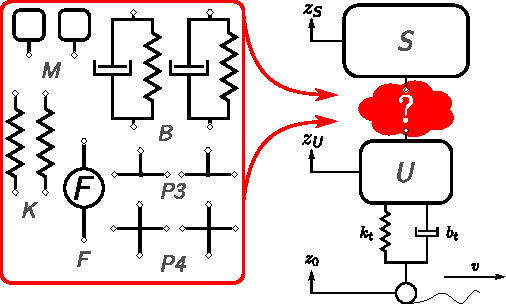
\includegraphics[width=0.55\columnwidth]{../ch8/figures/suspension1}
\caption{Suspension architecture component catalog.\label{fig:ch8:suspension1}}
\end{figure}

The component catalog and NSCs will be the same as the case study in Sec.~\ref{sec:ch2:example4}.
The $(\gls{C}, \gls{R}, \gls{P})$ specification is:
\begin{subequations}
\label{eq:ch8:CRP}
\begin{align}
C &= \{\xcolor{S}, \xcolor{U},  \xcolor{M},  \xcolor{K},  \xcolor{B},  \xcolor{F}, \xcolor{P3}, \xcolor{P4} \} \\
R &= \begin{bmatrix} 1,1,2,2,2,1,2,2 \end{bmatrix} \\
P &= \begin{bmatrix} 1,1,1,2,2,2,3,4 \end{bmatrix}
\end{align}
\end{subequations}

\noindent The catalog is represented in Fig.~\ref{fig:ch8:suspension1}.
Each of the component types fits in the bond graph modeling paradigm: $\{\xcolor{S}, \xcolor{U},  \xcolor{M}\}$ are \xcolor{I}-type storage nodes, \xcolor{K} is a \xcolor{C}-type storage node, \xcolor{B} is a subsystem containing a spring and damper in parallel (see Fig.~\ref{fig:ch8:suspension1}), and \xcolor{F} is an \xcolor{Se}-type effort source.
The remaining component types represent \xcolor{1}-junctions with a differing connection numbers.

% new paragraph
The architecture-only objective function term is the sum of the additional physical components (i.e.,~everything but \xcolor{S}, \xcolor{U}, and \xcolor{P}$x$):
\begin{align}
\Psi_a = \gls{weights}_a\left( \gls{number}_{\xcolor{M}} + n_{\xcolor{K}} + n_{\xcolor{B}} + n_{\xcolor{F}} \right)
\end{align}

\noindent where $w_a$ is the weighting coefficient.
This just one metric for complexity that we can use to look at tradeoffs between complexity and performance.

%--------------------------------------
\subsection{Co-Design Problem}

Three outputs will be needed to capture the co-design problem formulation:
\begin{align}
\bm{y} = \begin{bmatrix} z_{\xcolor{U}} \\ \ddot{z}_\xcolor{S} \\ z_\xcolor{S} \\ u \end{bmatrix}
\end{align}

\begin{subequations}
\noindent namely the unsprung mass position, sprung mass acceleration, unsprung mass position, and control.
The co-design objective function is the sum of several performance metrics:
\begin{align} \label{eq:ch8:susobj}
\Psi_d = \int_{t_0}^{t_f} \left( w_1 \left( y_1 - z_0 \right)^2 + w_2 y_2^2 + w_3 y_4^2 \right) dt
\end{align}

\noindent where the term $w_1 \left( y_1 - z_0 \right)^2$ captures the handling objective, $w_2 y_2^2$ represents the passenger comfort objective, and $w_3 y_4^2$ control effort objective (see Refs.~\cite{Allison2014b, Alyaqout2007b, Fathy2003a}).

% new paragraph
Next, the states of the system are initialized to their zero equilibrium position with the following simple bound constraint: 
\begin{align}
\bm{\xi}\xarch(t_0) = \bm{0} 
\end{align}

To ensure that the separation between the sprung and unsprung masses remains tolerable, the following rattlespace constraint is necessary \cite{Allison2014b, Fathy2003a, Gobbi2001a, Hrovat1993a, Ulsoy1994a}:
\begin{align}
\abs{y_3 - y_1} \leq \gls{rattlespace}
\end{align}

\noindent This constraint can be converted into two linear constraints as is shown in Sec.~\ref{sec:ch5:absolute:values}.
The rattlespace constraint is commonly included in the objective function but is more appropriately included as a constraint.
The LQDO problem class can readily handle linear inequality constraints unlike other solution strategies \cite{Allison2014b,manuscript-dt-qp}.

% new paragraph
All the previous constraints are necessary for the inner-loop co-design problem.
The outer-loop specific plant constraints are simple bounds on the linear coefficients:
\begin{align}
\gls{mass}_{\glsfoo[noindex]{min}} \leq \bm{x}_m\xarch \leq m_{\glsfoo[noindex]{max}} \\
\gls{damper}_{\min} \leq \bm{x}_b\xarch \leq b_{\max} \\
\gls{spring}_{\min} \leq \bm{x}_k\xarch \leq k_{\max} 
\end{align}

\noindent where the subscripts $\{m,b,k\}$ indicate the additional mass, damper, and spring plant variables for the candidate architecture.

\end{subequations}

\begin{table}
\centering
\begin{tabular}{cc|cc}
\hline \hline
Parameter & Value & Parameter & Value \\
\hline
$w_1$ & $10^5$ & $k_t$ & $232\times 10^3$ N/m \\
$w_2$ & $0.5$ & $b_t$ & $0$ Ns/m \\
$w_3$ & $10^{-5}$ & $r_{\max}$ & $0.03$ m \\
$t_0$ & $0$ s & $t_f$ & $9$ s \\
$m_{\min}$ & $0.001$ kg & $m_{\max}$ & $5$ kg  \\
$b_{\min}$ & $10^3$ Ns/m & $b_{\max}$ & $10^6$ Ns/m \\
$k_{\min}$ & $10^3$ N/m & $k_{\max}$ & $10^7$ N/m \\
$m_{\xcolor{U}}$ & $65$ kg & $m_{\xcolor{S}}$ & $325$ kg \\
\hline \hline
\end{tabular}
\caption{Co-design problem parameters.\label{tb:ch8:parameters}}
\end{table}

The problem parameters used in this study are shown in Table~\ref{tb:ch8:parameters} (many of the parameters are based the study in Ref.~\cite{Allison2014b}).
A rough road input is used from Refs.~\cite{Allison2008b, Allison2014b}.

\section{Results\label{sec:ch8:results}}

\begin{table}
\centering
\small

\begin{subfigure}[b]{\textwidth}
\centering
\caption{Maximum control and optimal plant variables.}
\begin{tabular}{ccccccc}
\hline \hline 
\# & Figure & $\Psi_a/w_a$ & $\Psi_d$ & $w_1 \left( y_1 - z_0 \right)^2$ & $w_2 y_2^2$ & $w_3 y_4^2$ \\
\hline 
1 & Fig.~\ref{fig:ch8:csuspension1} & 2 & 10.96 & 6.60 & 4.36 & 0.00 \\
2 & Fig.~\ref{fig:ch8:csuspension2} & 1 & 7.79 & 3.10 & 1.51 & 3.18 \\
3 & Fig.~\ref{fig:ch8:csuspension3} & 3 & 7.52 & 3.25 & 1.99 & 2.28 \\
4 & Fig.~\ref{fig:ch8:csuspension4} & 4 & 7.79 & 3.09 & 1.51 & 3.19 \\
5 & Fig.~\ref{fig:ch8:csuspension5} & 7 & 6.58 & 2.48 & 2.43 & 1.68 \\
6 & Fig.~\ref{fig:ch8:csuspension6} & 7 & 9.69 & 5.27 & 4.42 & 0.00 \\
\hline \hline 
\end{tabular}
\end{subfigure}%

\vspace{2px}

\begin{subfigure}[t]{\textwidth}
\centering
\caption{Maximum control and optimal plant variables.}
\begin{tabular}{cccccccccc}
\hline \hline 
\# & Figure & $\max{\abs{u}}$ & $k_1$ & $k_2$ & $k_3$ & $b_1$ & $b_2$ & $m_1$ & $m_2$ \\
\hline 
1 & Fig.~\ref{fig:ch8:csuspension1} & 0 & $1.77\textsc{e}4$ & $-$ & $-$ & $1.88\textsc{e}3$ & $-$ & $-$ & $-$ \\
2 & Fig.~\ref{fig:ch8:csuspension2} & 598 & $-$ & $-$ & $-$ & $-$ & $-$ & $-$ & $-$ \\
3 & Fig.~\ref{fig:ch8:csuspension3} & 634 & $1.47\textsc{e}4$ & $-$ & $-$ & $1.00\textsc{e}3$ & $-$ & $-$ & $-$ \\
4 & Fig.~\ref{fig:ch8:csuspension4} & 611 & $6.89\textsc{e}6$ & $-$ & $-$ & $6.04\textsc{e}5$ & $-$ & $1.02\textsc{e-}3$ & $-$ \\
5 & Fig.~\ref{fig:ch8:csuspension5} & 478 & $9.55\textsc{e}4$ & $6.67\textsc{e}3$ & $8.83\textsc{e}4$ & $1.46\textsc{e}4$ & $2.01\textsc{e}3$ & $3.11\textsc{e-}3$ & $-$ \\
6 & Fig.~\ref{fig:ch8:csuspension6} & 0 & $7.28\textsc{e}4$ & $8.54\textsc{e}3$ & $2.51\textsc{e}5$ & $1.00\textsc{e}3$ & $2.27\textsc{e}3$ & $3.21\textsc{e}0$ & $1.10\textsc{e}0$ \\
\hline \hline 
\end{tabular}
\end{subfigure}%

\caption{Summary of the suspension design results.\label{fig:ch8:results}}

\end{table}

In this section, we summarize the results of the vehicle suspension case study.
We utilize the code from Ref.~\cite{github-dt-qp-project} to solve the control subproblem.
The defect constraints are formed using the \glsfoo[noindex]{TR} and the chosen quadrature the \glsfoo[noindex]{CQHS} method (see Chapter~\ref{ch:5}).
It was determined that 2000 time points were needed to approximate sufficiently the problem.
The results for the first four architectures in Fig.~\ref{fig:ch8:suspensions} are presented in Table~\ref{fig:ch8:results}, along with the other two novel candidate suspensions.
A variety of stochastically generated suspensions were evaluated in the graph structure space defined by Prob.~(\ref{eq:ch8:CRP}), and the two reported novel architectures were the among the best performing for an active or passive suspension system.

% new paragraph
As expected, the worst-performing suspension of the six in Fig.~\ref{fig:ch8:suspensions} was the canonical passive design (some of the optimal position trajectories and the rattlespace are shown in Fig.~\ref{fig:ch8:results1}).
Here we see fairly large fluctuations in $z_{\xcolor{S}}$, and the rattlespace constraint is satisfied. 
The alternative passive suspension in Fig.~\ref{fig:ch8:csuspension6} (results in Fig.~\ref{fig:ch8:results6}) achieved a 12\% reduction in the objective function.
The primary improvement was in the handling objective.
However, this architecture is more complex with seven additional components compared the original two.

% new paragraph
The results for the pure active suspension are shown in Fig.~\ref{fig:ch8:results2}.
Compared to the passive suspensions, the performance index is significantly lower, demonstrating the potential value of an active component.
Since there are no passive components naturally keeping the sprung mass near the equilibrium position in this architecture, we see a drift in the sprung mass position (but the rattlespace constraint is still satisfied).
The canonical active suspension in Fig.~\ref{fig:ch8:csuspension3} does not have this issue. 
From the results in Fig.~\ref{fig:ch8:results3}, we see a very different profile for $z_{\xcolor{S}}$.
Since this architecture has some plant design flexibility, we expected an improvement in performance over the pure active design.
A 3.5\% decrease in the objective function value is observed indicating that the addition of the two passive components does result in a minor improvement in performance.
The distribution of the individual objective function terms in Eqn.~(\ref{eq:ch8:susobj}) is quite different between the two suspensions.

% new paragraph
The addition of the dynamic absorber to the pure active suspension in Fig.~\ref{fig:ch8:csuspension4} is supposed to improve handling without compromising the comfort objective \cite{Hrovat1993a}.
However, the results in Fig.~\ref{fig:ch8:results4} indicate no performance benefit for this architecture change with respect to the specific problem parameters used in this study.
This is most readily observed with the value of the additional mass  near the lower bound of 0.001 kg (effectively removing it from the system).
It is also the only architecture where the rattlespace constraint is active at some point during the time horizon.
The final architecture had the best overall performance with a 13\% reduction compared to the canonical active suspension.
The results are shown in Fig.~\ref{fig:ch8:results6}, and this design had the smallest maximum control effort.
Once again, the dynamic absorber subcomponent (now attached to the sprung mass) is ineffective with a mass value near the lower bound.
This design did need seven additional components to achieve this performance improvement.

\begin{figure}

\begin{subfigure}[b]{0.5\textwidth}
\centering
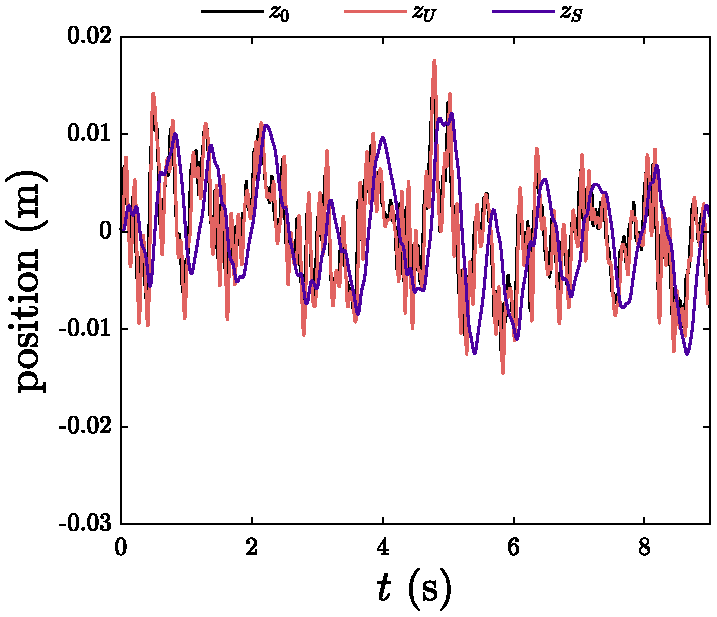
\includegraphics[width=\textwidth]{../ch8/figures/design3-position}
% 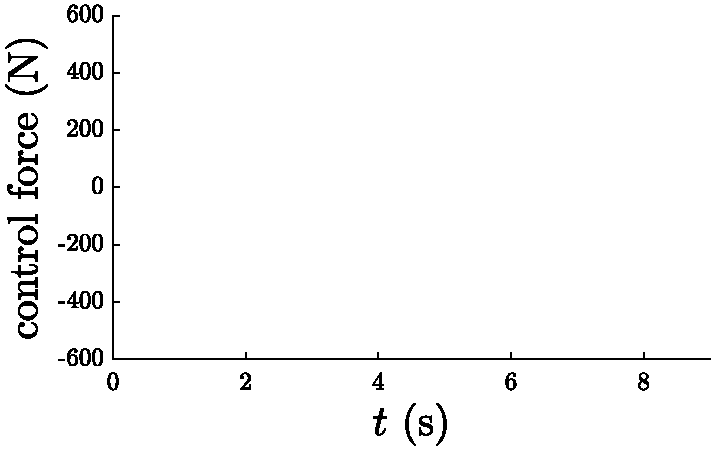
\includegraphics[width=\textwidth]{../ch8/figures/design3-control}
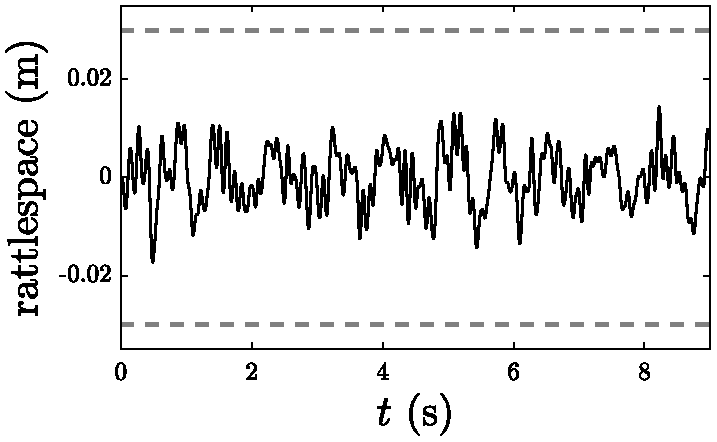
\includegraphics[width=\textwidth]{../ch8/figures/design3-rattlespace}
\caption{Canonical passive in Fig.~\ref{fig:ch8:csuspension1}.\label{fig:ch8:results1}}
\end{subfigure}%
\begin{subfigure}[b]{0.5\textwidth}
\centering
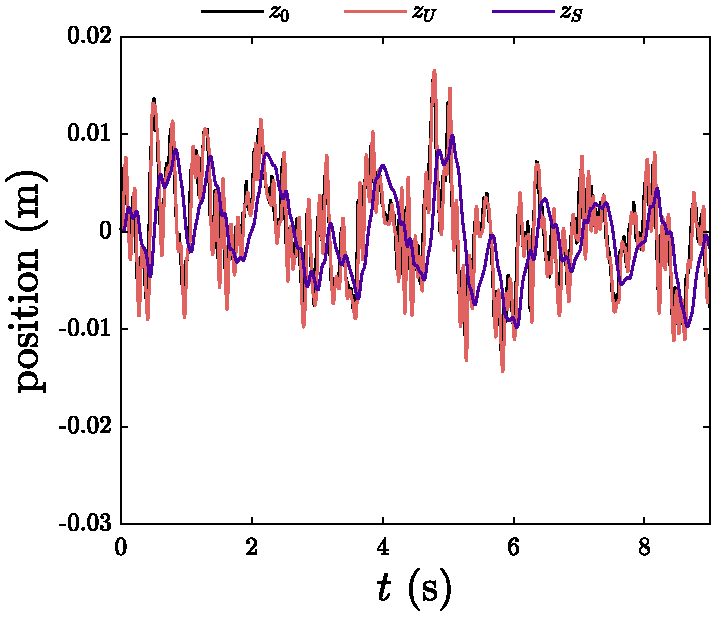
\includegraphics[width=\textwidth]{../ch8/figures/design6-position}
% 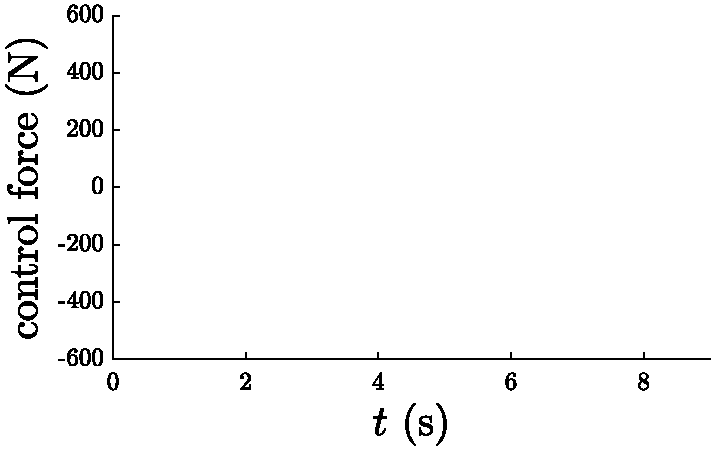
\includegraphics[width=\textwidth]{../ch8/figures/design6-control}
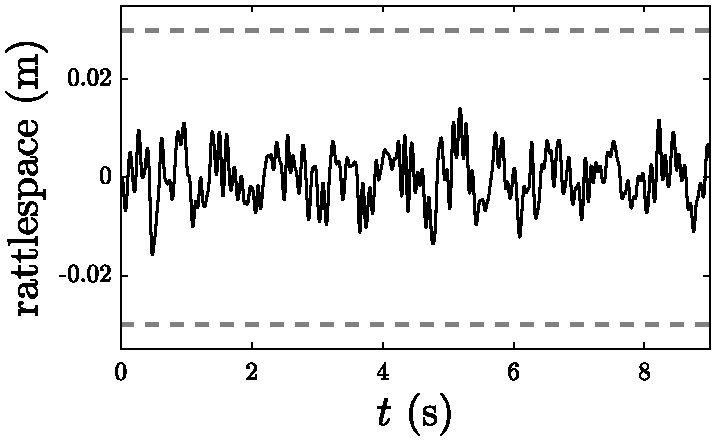
\includegraphics[width=\textwidth]{../ch8/figures/design6-rattlespace}
\caption{Passive candidate in Fig.~\ref{fig:ch8:csuspension6}.\label{fig:ch8:results6}}
\end{subfigure}%

\caption{Optimal trajectories for the two passive suspensions.}

\end{figure}

\begin{figure}

\begin{subfigure}[b]{0.5\textwidth}
\centering
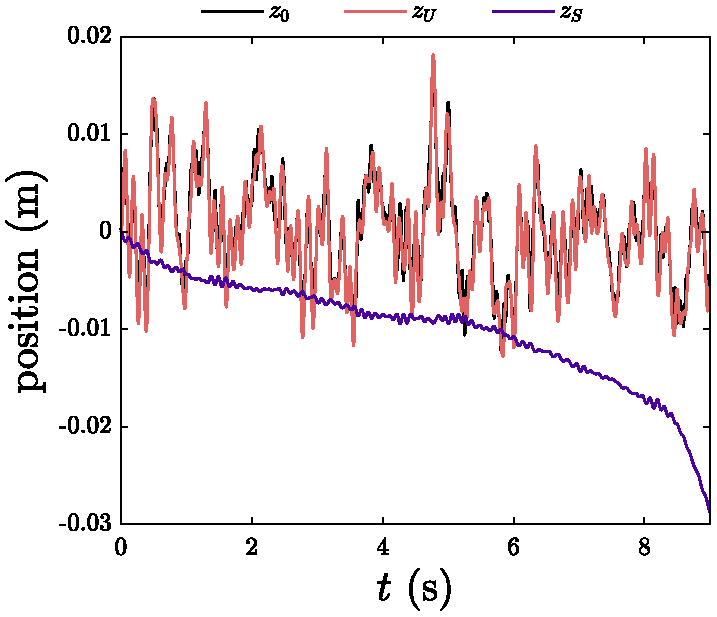
\includegraphics[width=\textwidth]{../ch8/figures/design2-position}
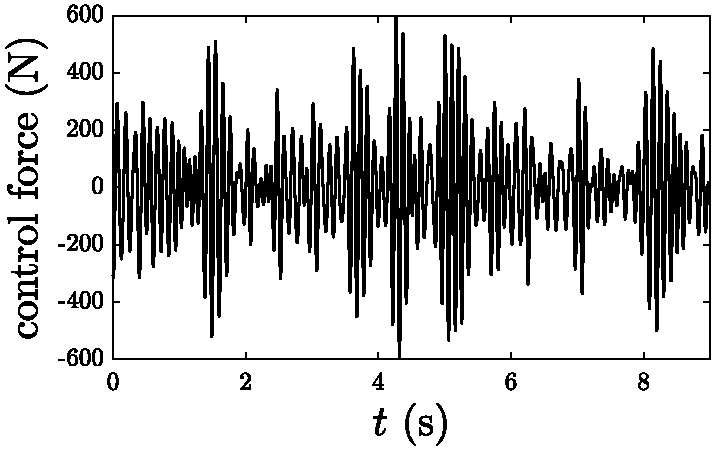
\includegraphics[width=\textwidth]{../ch8/figures/design2-control}
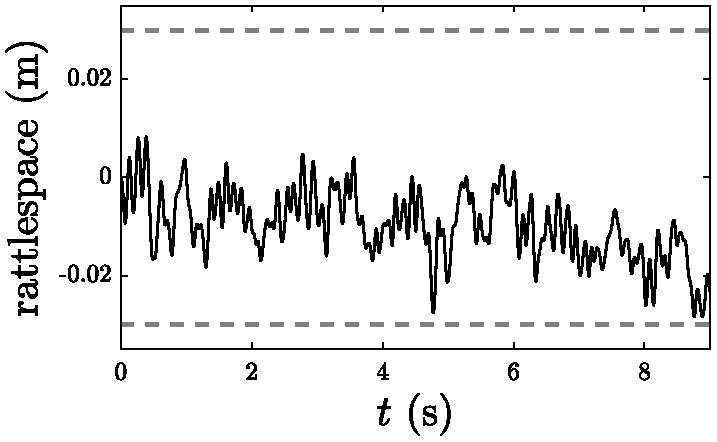
\includegraphics[width=\textwidth]{../ch8/figures/design2-rattlespace}
\caption{Pure active in Fig.~\ref{fig:ch8:csuspension2}.\label{fig:ch8:results2}}
\end{subfigure}%
\begin{subfigure}[b]{0.5\textwidth}
\centering
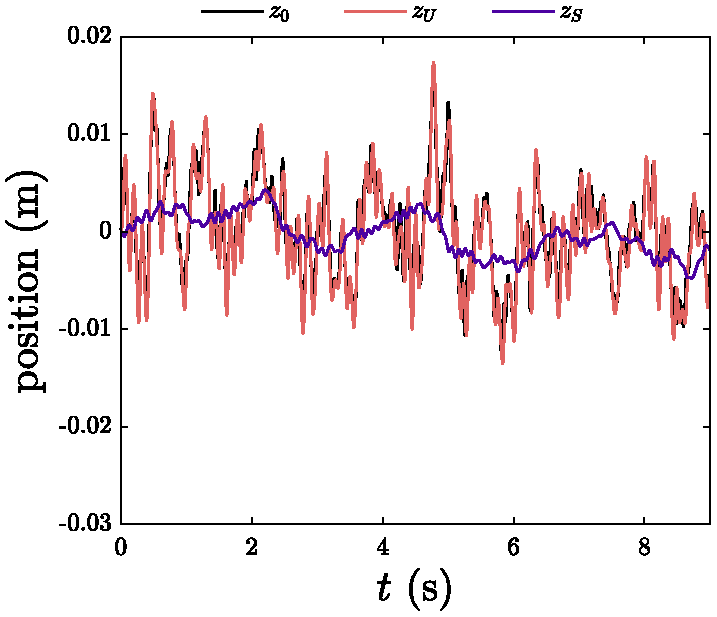
\includegraphics[width=\textwidth]{../ch8/figures/design1-position}
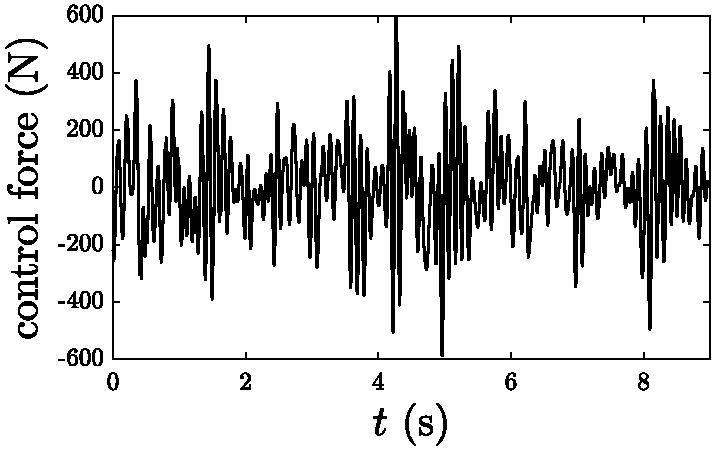
\includegraphics[width=\textwidth]{../ch8/figures/design1-control}
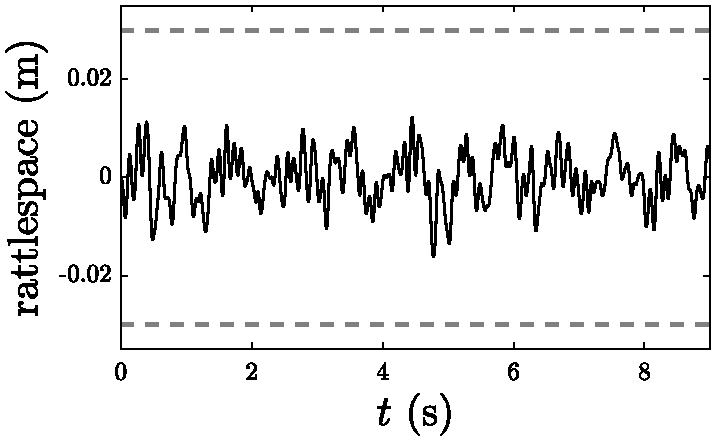
\includegraphics[width=\textwidth]{../ch8/figures/design1-rattlespace}
\caption{Canonical active in Fig.~\ref{fig:ch8:csuspension3}.\label{fig:ch8:results3}}
\end{subfigure}%

\caption{Optimal trajectories for two suspensions.}

\end{figure}

\begin{figure}

\begin{subfigure}[b]{0.5\textwidth}
\centering
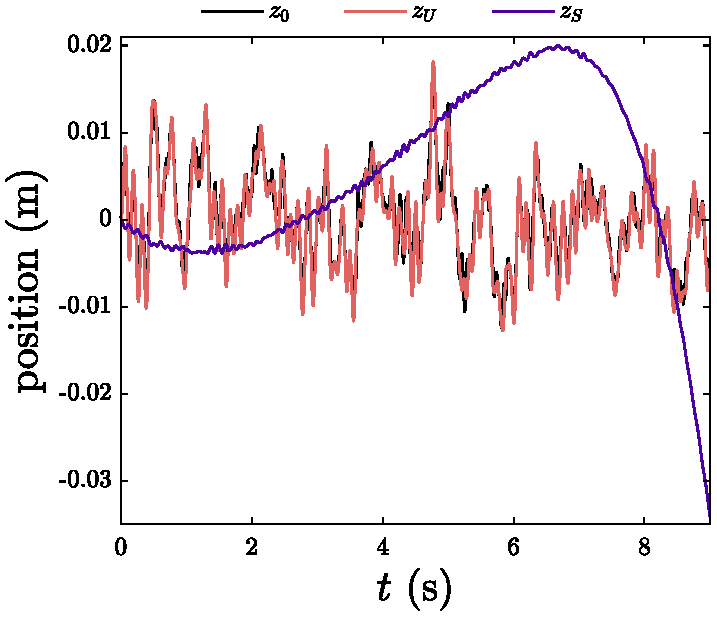
\includegraphics[width=\textwidth]{../ch8/figures/design4-position}
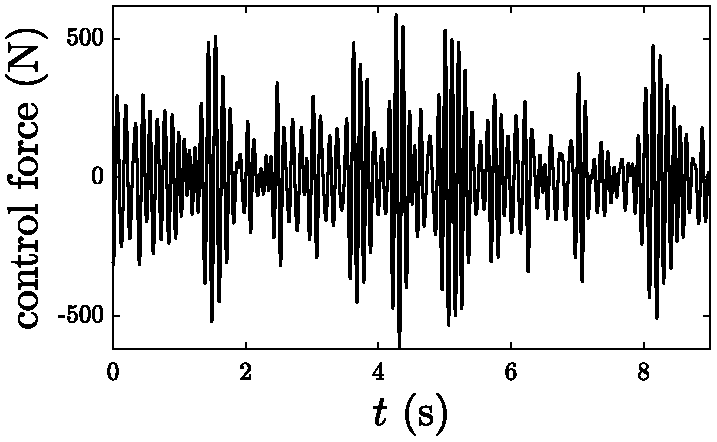
\includegraphics[width=\textwidth]{../ch8/figures/design4-control}
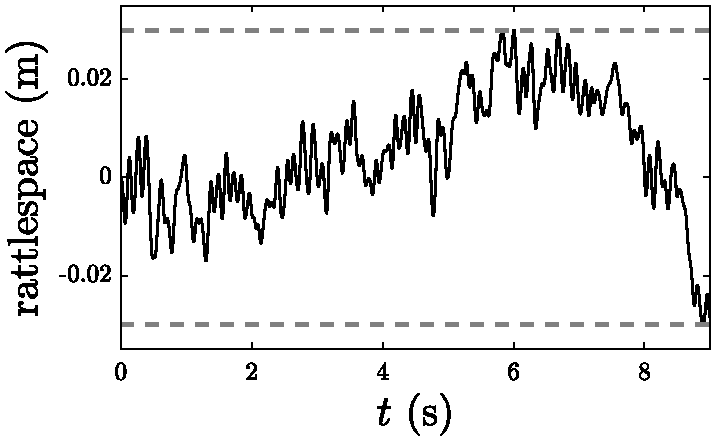
\includegraphics[width=\textwidth]{../ch8/figures/design4-rattlespace}
\caption{Active with dynamic absorber in Fig.~\ref{fig:ch8:csuspension4}.\label{fig:ch8:results4}}
\end{subfigure}%
\begin{subfigure}[b]{0.5\textwidth}
\centering
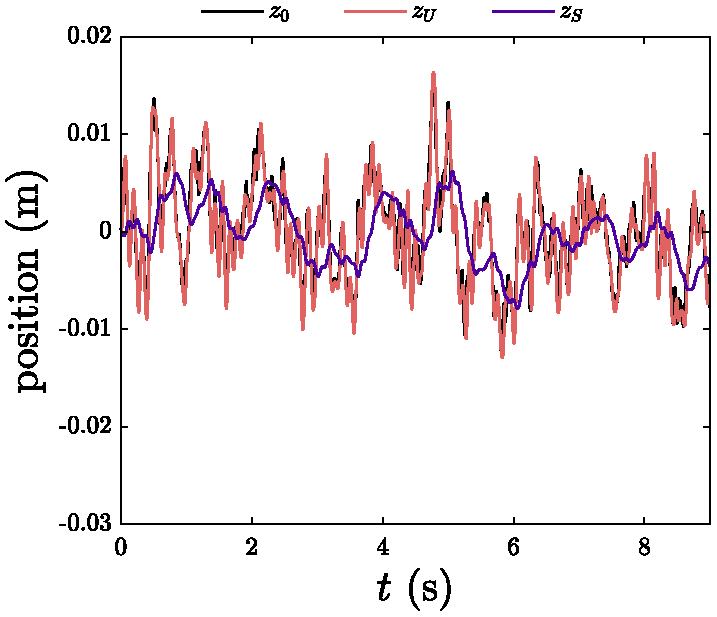
\includegraphics[width=\textwidth]{../ch8/figures/design5-position}
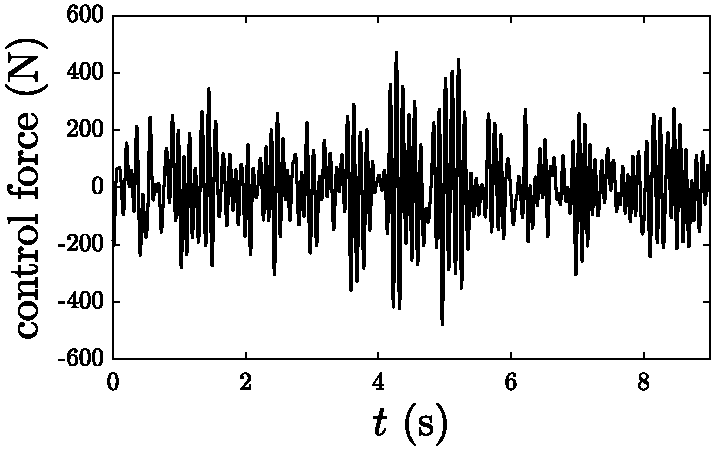
\includegraphics[width=\textwidth]{../ch8/figures/design5-control}
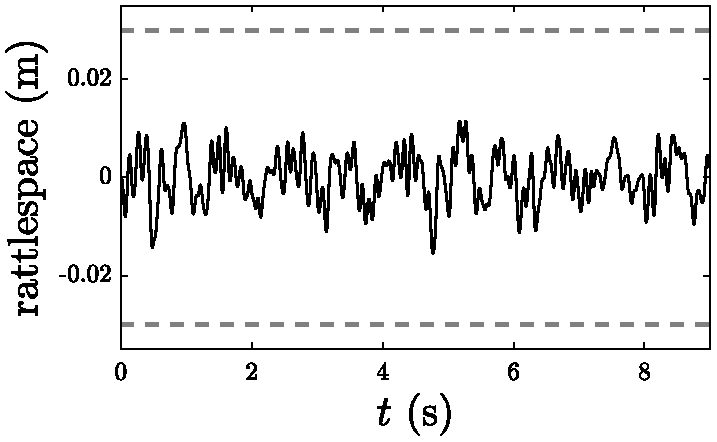
\includegraphics[width=\textwidth]{../ch8/figures/design5-rattlespace}
\caption{Active candidate in Fig.~\ref{fig:ch8:csuspension5}.\label{fig:ch8:results5}}
\end{subfigure}%

\caption{Optimal trajectories for two suspensions including the current best architecture.}

\end{figure}

\section{Summary\label{sec:ch8:conclusion}}

The results in this case study demonstrate that changes to the vehicle suspension architecture can result in improved performance.
The purpose of these early-stage studies is to identify new architectures that could be investigated in the same level of detail that the few canonical architectures have received.
This case study utilized a newly developed paradigm for combined architecture, plant, and control design that can be applied to systems with linear physical elements.

% new paragraph
It remains future work to evaluate the entire set of possible 13,727 unique suspension architectures from Prob.~(\ref{eq:ch8:CRP}) \cite{Herber2017a}.
In addition, there are a number of improvements that can be made to the problem formulation.
Multiple road inputs should be considered simultaneously to give a better representation of all the environments the suspension will need to function in.
Frequency domain properties, such as suspension quality spectral density and control energy spectral density, could also be utilized for a more effective problem formulation  \cite{Fathy2003a}.